% $Header: /cvsroot/latex-beamer/latex-beamer/solutions/conference-talks/conference-ornate-20min.en.tex,v 1.6 2004/10/07 20:53:08 tantau Exp $

\documentclass{beamer}

\mode<presentation>
{
%  \usetheme{Hannover}
\usetheme[width=0.7in]{Hannover}
% or ...

  \setbeamercovered{transparent}
  % or whatever (possibly just delete it)
}
\usepackage{longtable}
\usepackage{booktabs}

\usepackage[english]{babel}
% or whatever

\usepackage[latin1]{inputenc}
% or whatever

\usepackage{times}
%\usepackage[T1]{fontenc}
% Or whatever. Note that the encoding and the font should match. If T1
% does not look nice, try deleting the line with the fontenc.
%\usepackage{logictheme}

%\usepackage{hhline}
\usepackage{multirow}
%\usepackage{multicol}
%\usepackage{array}
%\usepackage{supertabular}
%\usepackage{amsmath}
%\usepackage{amsfonts}
\usepackage{totpages}
\usepackage{hyperref}
%\usepackage{booktabs}

%\usepackage{bm}

\usepackage{listings}
\usepackage{color}
 
\definecolor{codegreen}{rgb}{0,0.6,0}
\definecolor{codegray}{rgb}{0.5,0.5,0.5}
\definecolor{codepurple}{rgb}{0.58,0,0.82}
\definecolor{backcolour}{rgb}{0.95,0.95,0.92}
 
\lstdefinestyle{mystyle}{
    backgroundcolor=\color{backcolour},   
    commentstyle=\color{codegray},
    keywordstyle=\color{magenta},
    numberstyle=\tiny\color{codegreen},
    stringstyle=\color{codepurple},
    basicstyle=\tiny,
    breakatwhitespace=false,         
    breaklines=true,                 
    captionpos=b,                    
    keepspaces=true,                 
    numbers=left,                    
    numbersep=5pt,                  
    showspaces=false,                
    showstringspaces=false,
    showtabs=false,                  
    tabsize=2
}
 
\lstset{style=mystyle}
\newcommand{\blt}{- } %used for bullets in a list

\newcounter{datadefnum} %Datadefinition Number
\newcommand{\ddthedatadefnum}{DD\thedatadefnum}
\newcommand{\ddref}[1]{DD\ref{#1}}

\newcommand{\colAwidth}{0.2\textwidth}
\newcommand{\colBwidth}{0.73\textwidth}

\newcommand{\red}{\textcolor{red}}
\newcommand{\ro}[1]{\only<#1>{\red}}

\renewcommand{\arraystretch}{0.6} %so that tables with equations do not look crowded

\pgfdeclareimage[height=0.7cm]{logo}{McMasterLogo}
\pgfdeclareimage[width=10.55cm]{ex1}{h_g_ex}
\pgfdeclareimage[width=6cm]{rec1}{SRS_ex}
\pgfdeclareimage[width=6cm]{rec2}{LPM_ex}
\title[\pgfuseimage{logo}]  % (optional, use only with long paper titles)
{PhD Committee Meeting \#4}

%\subtitle
%{Include Only If Paper Has a Subtitle}

\author[Slide \thepage~of \pageref{TotPages}] % (optional, use only with lots of
                                              % authors)
{Dan Szymczak}
% - Give the names in the same order as the appear in the paper.
% - Use the \inst{?} command only if the authors have different
%   affiliation.

\institute[McMaster University] % (optional, but mostly needed)
{
  Computing and Software Department\\
  Faculty of Engineering\\
  McMaster University
}
% - Use the \inst command only if there are several affiliations.
% - Keep it simple, no one is interested in your street address.

\date[June 28, 2018] % (optional, should be abbreviation of conference name)
{June 28, 2018}
% - Either use conference name or its abbreviation.
% - Not really informative to the audience, more for people (including
%   yourself) who are reading the slides online

% If you have a file called "university-logo-filename.xxx", where xxx
% is a graphic format that can be processed by latex or pdflatex,
% resp., then you can add a logo as follows:

%\pgfdeclareimage[height=0.5cm]{Mac-logo}{McMasterLogo}
%\logo{\pgfuseimage{Mac-logo}}

% Delete this, if you do not want the table of contents to pop up at
% the beginning of each subsection:
\AtBeginSubsection[]
{
  \begin{frame}<beamer>
    \frametitle{Outline}
    \tableofcontents[currentsection,currentsubsection]
  \end{frame}
}

% If you wish to uncover everything in a step-wise fashion, uncomment
% the following command: 

%\beamerdefaultoverlayspecification{<+->}

\beamertemplatenavigationsymbolsempty 

% have SRS and LP open during the presentation

\begin{document}

%%%%%%%%%%%%%%%%%%%%%%%%%%%%%%%%%%%%%%
\begin{frame}

\titlepage

\end{frame}

%%%%%%%%%%%%%%%%%%%%%%%%%%%%%%%%%%%%%%

\begin{frame}

\frametitle{Overview}
\tableofcontents
% You might wish to add the option [pausesections]

% make like a story - the phases - reason for, why works, advantages
% changing the history a bit to make a more rational narrative

\end{frame}

%%%%%%%%%%%%%%%%%%%%%%%%%%%%%%%%%%%%%%
%
%\section[Introduction]{Introduction}
%
%% \subsection[Important Software Qualities]{Scientific Computing Software
%% Qualities}

%%%%%%%%%%%%%%%%%%%%%%%%%%%%%%%%%%%%%%

%\begin{frame}
%
%\frametitle{Who am I?}
%
%Dan Szymczak
%
%\vspace{0.5cm}
%\pgfuseimage{Dan2}\hspace{1cm}\pgfuseimage{Dan}
%\end{frame}

%%%%%%%%%%%%%%%%%%%%%%%%%%%%%%%%%%%%%%

%\begin{frame}
%
%\frametitle{Education History}
%
%\begin{itemize}
%\item Ph.D. Software Engineering
%	\begin{itemize}
%	\item Currently in progress. Started Autumn 2014.
%	\end{itemize}
%\item M.A.Sc. Software Engineering
%	\begin{itemize}
%	\item McMaster University 2014
%	\item Thesis -- \textit{Generating Learning Algorithms: Hidden Markov Models as a Case Study}
%	\end{itemize}
%\item B.Eng Software (Game Design) 
%\begin{itemize}
%	\item McMaster University 2011
%	\end{itemize}
%
%\end{itemize}
%\end{frame}
%%%%%%%%%%%%%%%%%%%%%%%%%%%%%%%%%%%%%%

\section[Recap]{Research Recap}

%%%%%%%%%%%%%%%%%%%%%%%%%%%%%%%%%%%%%%

\begin{frame}
\setbeamercovered{invisible}
\frametitle{Research Topic Recap}
\framesubtitle{\alt<6->{\ro{6}{KBSE \& The Drasil Framework}}{Motivation}}

\only<6->{\ro{6}{A Knowledge-Based Software Engineering Approach}}
\begin{itemize}
	\item<1->\alt<7->{\ro{7}{Single knowledge-base}}{Too much 
	duplication!}
	\item<2->\alt<8->{\ro{8}{Generate artifacts}}{(Re-)Certification is 
	expensive}
	\item<3->\alt<9->{\ro{9}{Guaranteed consistency}}{Inter-/intra-artifact 
	consistency 
	issues}% \& improve:
%		\begin{itemize}
%			\item Verifiability
%			\item Maintainability
%			\item Reusability
%		\end{itemize}
	\item<4->\alt<10->{\ro{10}{Reusable across projects}}{Promote reusability}
	\item<5->\alt<11->{\ro{11}{Easy to mix and match}}{Design for change} %-- 
	%Easily 
	%switch between software family members
\end{itemize}

\end{frame}

%%%%%%%%%%%%%%%%%%%%%%%%%%%%%%%%%%%%%%

%\begin{frame}
%
%\frametitle{Research Topic Recap}
%\framesubtitle{KBSE \& The Drasil Framework}
%
%A Knowledge-Based Software Engineering Approach
%\setbeamercovered{invisible}
%\begin{itemize}
%	\item<2->\alt<3->{Single knowledge-base}{Too much duplication!}
%	\item<4->\alt<5->{Generate artifacts}{(Re-)Certification is expensive}
%	\item<6->\alt<7->{Guaranteed consistency}{Inter-/intra-artifact consistency 
%	issues}% \& improve:
%	\item<8->\alt<9->{Reusable across projects}{Promote reusability}
%	\item<10->\alt<11->{Easy to mix and match}{Design for change} %-- Easily 
%	%switch between software family members
%\end{itemize}
%
%\end{frame}

\begin{frame}
\frametitle{Research Topic Recap}
\framesubtitle{KBSE \& The Drasil Framework}

\only<1-2>{Drasil -- Towards generating Software Families}

\only<1>{
\begin{center}
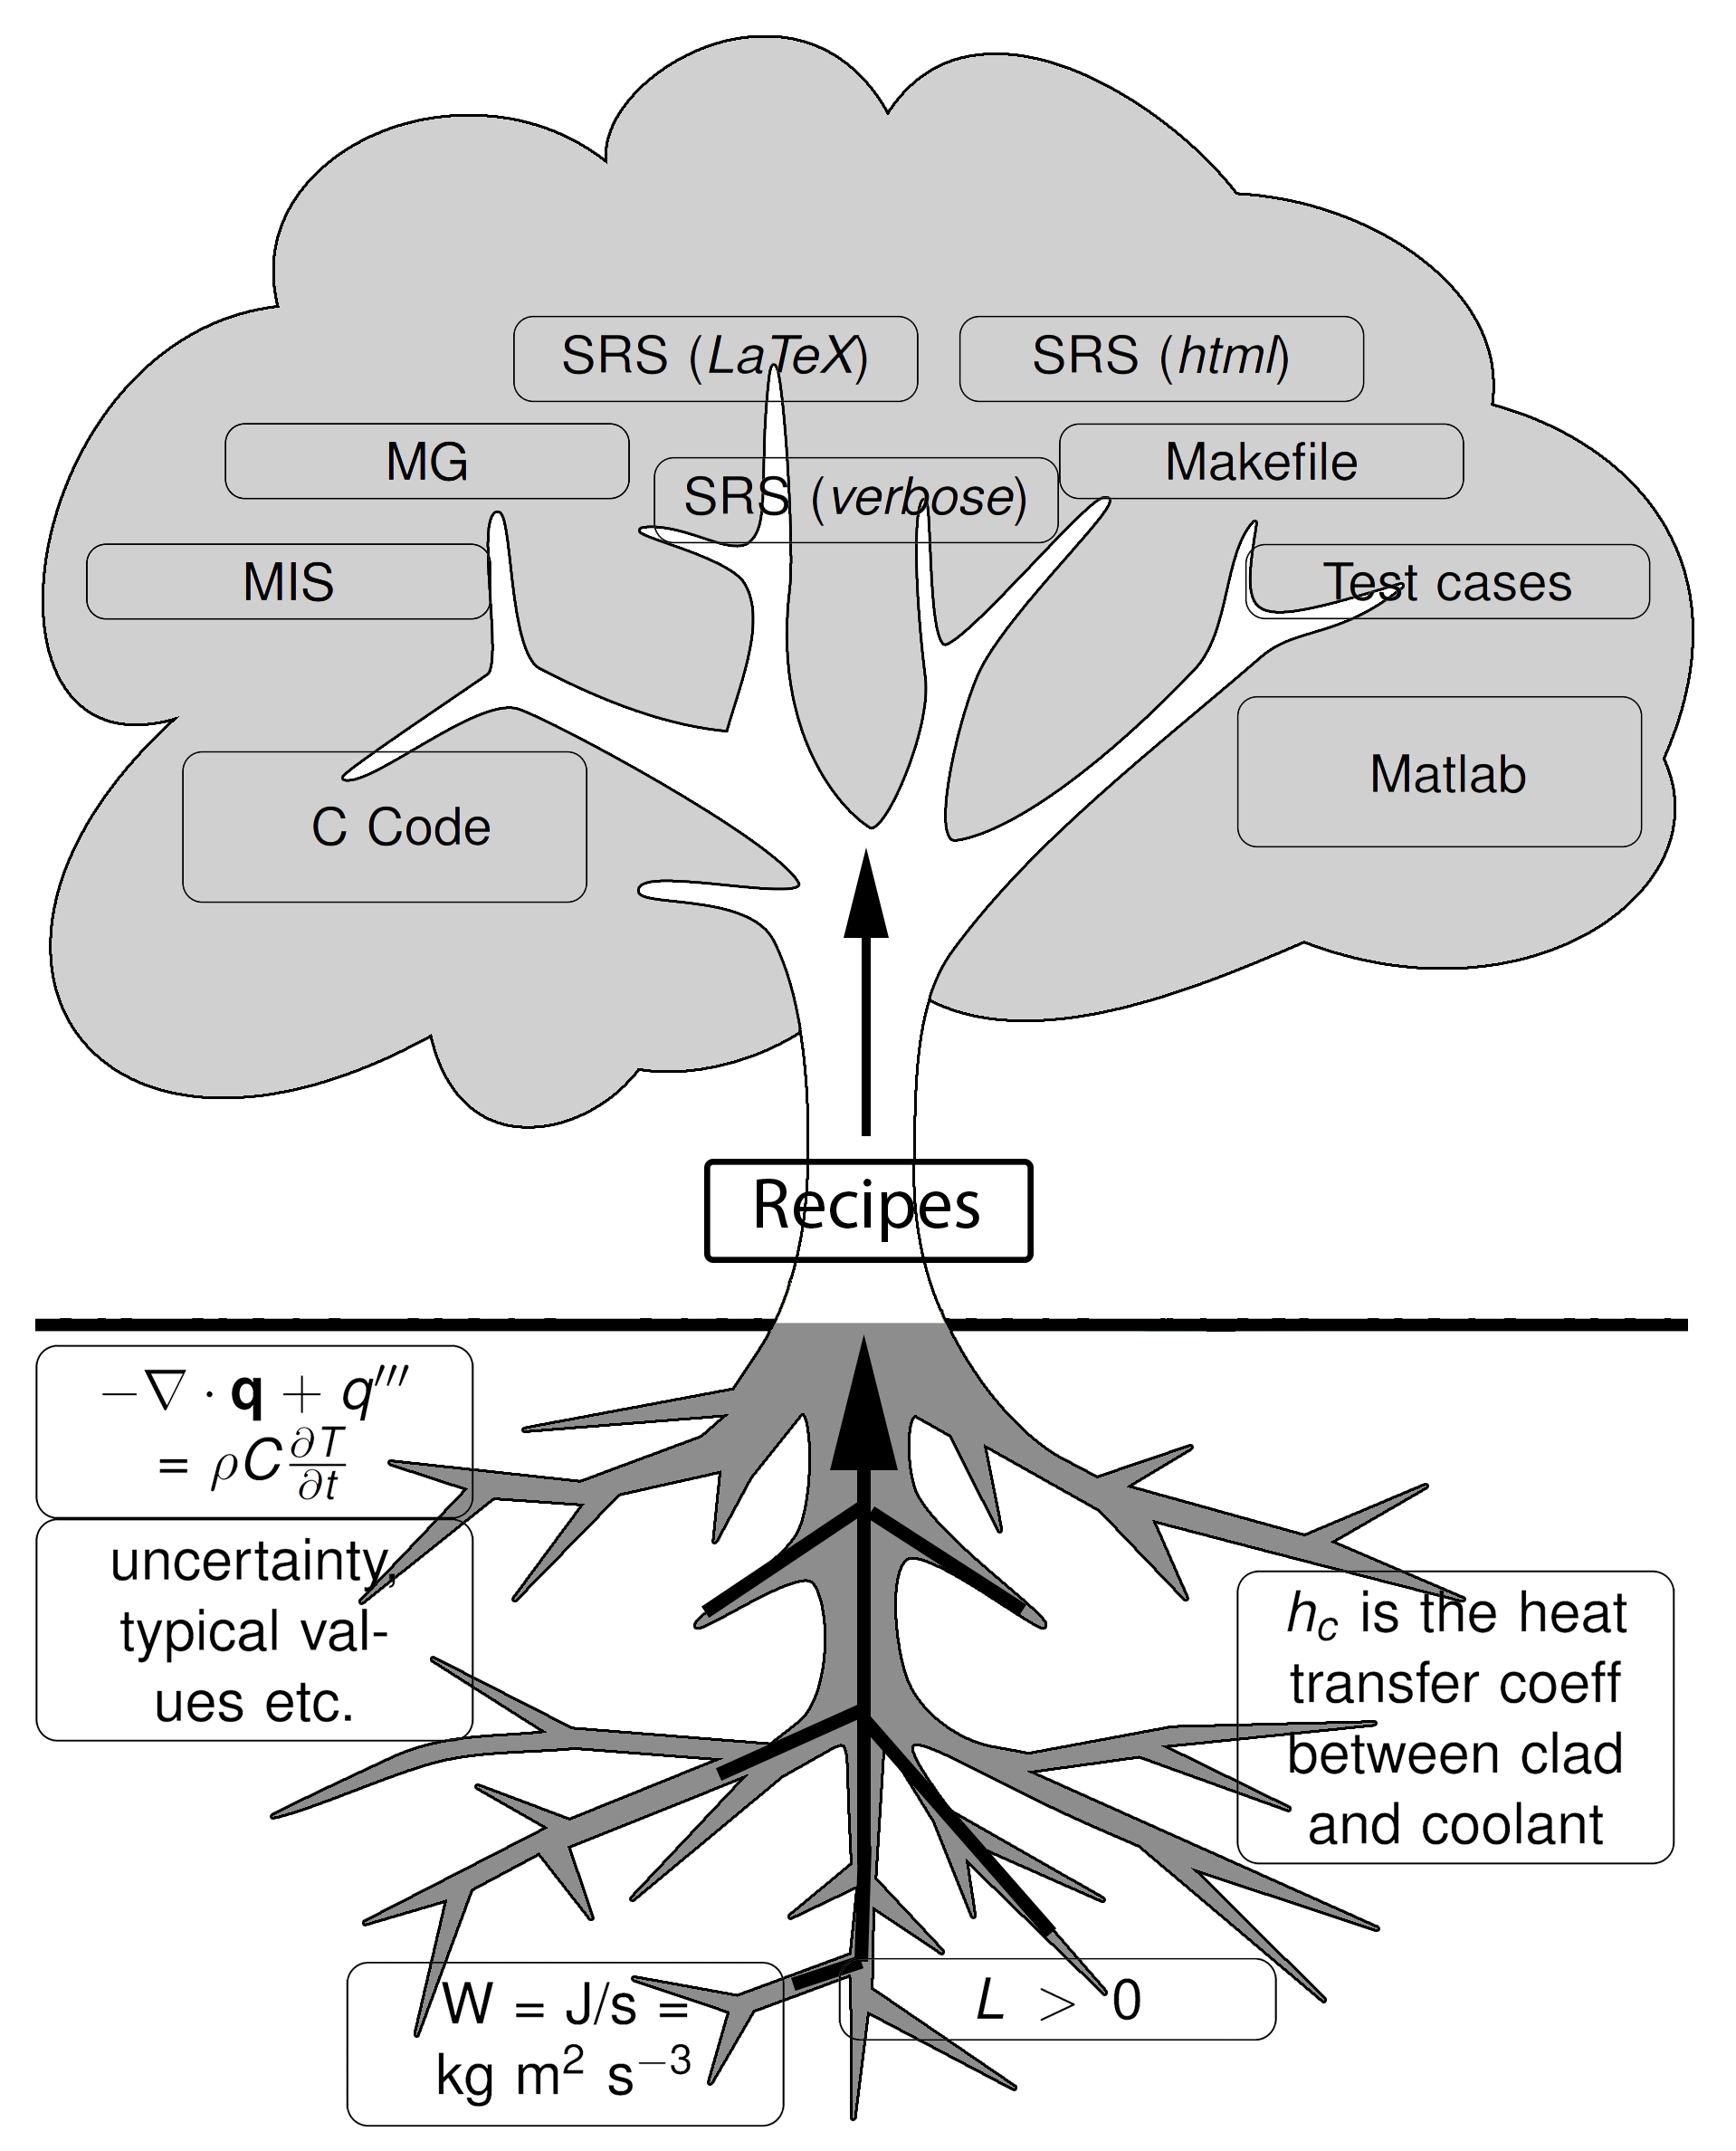
\includegraphics[scale=0.07]{tree.png}
\end{center}
}

\only<2>{
\begin{itemize}
	\item One ``source'', multiple views
	\item Full traceability
	\item Consistent-by-construction artifacts
\end{itemize}
}

\only<3>{
Drasil composed of many Domain-Specific Languages (DSLs) including, but not 
limited to:
\begin{itemize}
\item Knowledge Capture
\item Recipes (Document generation)
\item Code Generation
\end{itemize}
}
\end{frame}

%%%%%%%%%%%%%%%%%%%%%%%%%%%%%%%%%%%%%%%

\section[Progress]{Current Progress}

%%%%%%%%%%%%%%%%%%%%%%%%%%%%%%%%%%%%%%%

\begin{frame}

\frametitle{Current Program Progress}
\framesubtitle{A brief overview \only<2>{continued}}

\only<1>{
\begin{itemize}
\item Completed all necessary graduate courses \& comprehensive examinations
%	\begin{itemize}
%	\item CAS781 -- Category Theory: A (11)
%	\item CAS703 -- Software Design: A (11)
%	\item CAS708 -- Scientific Computation: A+ (12)
%	\item CAS761 -- Generative Programming: A+ (12)
%	\end{itemize}

\item Currently Writing:
	\begin{itemize}
	\item Journal paper for ACM TOSEM
	%	\begin{itemize}
	%		\item Focus on (re-)certification and consistency
	%	\end{itemize}
	\item Thesis
	\end{itemize}
\end{itemize}
}

\only<2>{

Research Project: Drasil proof-of-concept ``complete"
\begin{itemize}
	\item Scoped-down due to nature of project
	\item Generating SRS for six case studies \& code for one
	\item Still improving with the help of summer students
% Work still being done is 2-part:
% 1. (Obv) For future researchers/students
% 2. To help me write -- If I can't explain something well-enough, it's usually 
%		because the code needs work
\end{itemize}

}
\end{frame}

%%%%%%%%%%%%%%%%%%%%%%%%%%%%%%%%%%%%%%

\begin{frame}

\frametitle{Since Last Time}
\only<1>{

\framesubtitle{General}
Summer 2017: Supervised 5 research students
\begin{itemize}
\item Cleaned up case studies
\item Helped improve Drasil
\end{itemize}

Submitted a paper for SE-CoDeSE'17: Rejected

Began work on a paper for FASE 2018 -- Scrapped

Met with OPG in January: Positive feedback

Currently co-supervising 3 summer research students

Writing %mentioned earlier
}

\only<2>{
\framesubtitle{Drasil-Specific}

Total of 372 issues closed on the Drasil github

\begin{itemize}
\item Haddock % Automated generation of some Drasil user-documentation using 
%Haddock
\item Chunk and referencing databases %improved referencing
\item Improved the Drasil class hierarchy %Added to, and refactored, 
% Citations, Theories, Labels, etc.
\item Finished creating Document Language (Cont'd)
\item Continuous Integration \& automated tests
\item General source clean-up and refactoring
\end{itemize}

Currently $\sim$130 open issues guiding development
}
\end{frame}

%%%%%%%%%%%%%%%%%%%%%%%%%%%%%%%%%%%%%%%

\begin{frame}
\frametitle{Document Language}

\only<1>{
\framesubtitle{Old}

\lstinputlisting[language=Haskell, firstline=46, lastline=75]{BodyOld.hs}

}

\only<2>{
\framesubtitle{New}
\lstinputlisting[language=Haskell, firstline=92, lastline=121]{BodyNew.hs}
}


\end{frame}

%%%%%%%%%%%%%%%%%%%%%%%%%%%%%%%%%%%%%%%
%
%\section[Example]{Example.}
%
%%%%%%%%%%%%%%%%%%%%%%%%%%%%%%%%%%%%%%%
%
%\begin{frame}
%
%\frametitle{Example: $h_g$}
%
%\framesubtitle{A simple example taken from the SRS for FP}
%
%$h_g$ is a symbol which appears in several locations including:
%\begin{itemize}
%\item The Software Requirements Specification
%\item The Literate Programmer's Manual
%\item The Source Code
%\end{itemize}
%
%Let's take a look!
%
%\end{frame}
%
%%%%%%%%%%%%%%%%%%%%%%%%%%%%%%%%%%%%%%%
%
%\begin{frame}
%
%\frametitle{Example: $h_g$}
%
%\framesubtitle{SRS Definition for $h_g$ (original)}
%
%\noindent
%\begin{minipage}{\textwidth}
%\begin{tabular}{p{\colAwidth} p{\colBwidth}}
%\toprule
%\textbf{Number} & \textbf{DD\refstepcounter{datadefnum}\thedatadefnum} 
%\label{hg}\\
%\midrule
%Label & $h_g$\\
%\midrule
%Units & $ML^0t^{-3}T^{-1}$\\
%\midrule
%SI & $\mathrm{\frac{kW}{m^{2} (^{\circ}C)}}$\\
%\midrule
%Equation & $h_g$ =$ \frac{2k_{c}h_{p}}{2k_{c}+\tau_c h_{p}}$\\
%\midrule
%Description & $h_g$ is the  gap conductance\newline
%$\tau_c$ is the clad thickness\newline
%$h_p$ is initial gap film conductance\newline
%$k_c$ is the clad conductivity\newline
%NOTE: Equation taken from the code\\
%\midrule
%Sources & source code\\
%\bottomrule
%\end{tabular}
%\end{minipage}\\
%
%\end{frame}
%
%%%%%%%%%%%%%%%%%%%%%%%%%%%%%%%%%%%%%%%
%
%\begin{frame}[fragile]
%
%\frametitle{Example: $h_g$}
%
%\framesubtitle{LPM Definition for $h_g$ (original)}
%
%\begin{equation} 
%h_{g} =\frac{2k_{c}h_{p}}{2k_{c}+\tau_c h_{p}}
%\end{equation}
%
%The corresponding C code is given by:
%
%\begin{lstlisting}[basicstyle=\tiny]
%double calc_hg(double k_c,double h_b,double tau_c)
%{
% return (2*(k_c)*(h_p)) / ((2*(k_c)) + (tau_c*(h_p)));
%}
%\end{lstlisting}
%
%\end{frame}
%
%%%%%%%%%%%%%%%%%%%%%%%%%%%%%%%%%%%%%%%
%
%%\begin{frame}
%%
%%\frametitle{Example: $h_g$ and $h_c$}
%%
%%\framesubtitle{Code source for $h_g$}
%%
%%\end{frame}
%
%%%%%%%%%%%%%%%%%%%%%%%%%%%%%%%%%%%%%%%
%
%\begin{frame}
%
%\frametitle{Example: $h_g$}
%
%\framesubtitle{A simple example taken from the SRS for FP}
%
%Modifying $h_g$ to reflect changes in requirements is not a simple
%matter. It involves, at the very least, the following steps:
%\begin{itemize}
%\item Update the definition in the SRS, LPM, and all other documents which
%  reference the symbol
%\item Modify the source code to reflect the new requirements
%\item Trace all dependencies
%\item Modify dependents to accomodate the change
%\item Ensure each of the documents is now up to date and consistent
%\end{itemize}
%
%\end{frame}
%
%%%%%%%%%%%%%%%%%%%%%%%%%%%%%%%%%%%%%%%
%
%\begin{frame}
%
%\frametitle{Example: $h_g$}
%
%\framesubtitle{Simplifying the process}
%
%%This is where knowledge capture comes into play. 
%Here is an example of a ``chunk'' for $h_g$:
%
%\pgfuseimage{ex1}
%
%\end{frame}
%
%%%%%%%%%%%%%%%%%%%%%%%%%%%%%%%%%%%%%%%
%
%\begin{frame}
%
%\frametitle{Example: $h_g$}
%
%\framesubtitle{How do we generate?}
%What do we do with the ``chunk''?
%
%That depends on the ``recipe''!
%
%\begin{itemize}
%\item To create our SRS we use the following recipe:
%\end{itemize}
%
%\pgfuseimage{rec1}
%
%\begin{itemize}
%\item To create our LPM we use the following recipe:
%\end{itemize}
%
%\pgfuseimage{rec2}
%
%\end{frame}
%
%%%%%%%%%%%%%%%%%%%%%%%%%%%%%%%%%%%%%%%
%
%\begin{frame}
%
%\frametitle{Example: $h_g$}
%
%\framesubtitle{Generated SRS Output}
%
%%Let's look at (excerpts of the) generated output:
%
%\noindent \begin{minipage}{\textwidth}
%\begin{tabular}{p{\colAwidth} p{\colBwidth}}
%\toprule \textbf{Number} & \textbf{DD\refstepcounter{datadefnum}\thedatadefnum}
%\label{hg}\\ \midrule
%Label & $h_{g}$\\ \midrule
%Units & $ML^0t^{-3}T^{-1}$\\ \midrule
%SI & $\mathrm{\frac{kW}{m^{2\circ} C}}$\\
%\midrule Equation & $h_{g}$ = $\frac{2k_{c}h_{p}}{2k_{c}+\tau_{c}h_{p}}$\\ 
%\midrule
%Description & $h_{g}$ is the effective heat transfer coefficient between clad 
%and fuel surface
%\newline
%$k_{c}$ is the
%clad conductivity \newline
%$h_{p}$ is the
%initial gap film conductance \newline
%$\tau_{c}$ is the
%clad thickness \newline
%NOTE: Equation taken from the code\\ \midrule
%Sources & source code\\
%\bottomrule \end{tabular} \end{minipage}\\
%\end{frame}
%
%%%%%%%%%%%%%%%%%%%%%%%%%%%%%%%%%%%%%%%
%
%\begin{frame}[fragile]
%
%\frametitle{Example: $h_g$}
%
%\framesubtitle{Generated LPM Output}
%
%%Let's look at (excerpts of the) generated output:
%
%\begin{equation}
%h_{g} =\frac{2k_{c}h_{p}}{2k_{c}+\tau_{c}h_{p}}\label{eq:hg}
%\end{equation}
%
%The corresponding C code is given by:
%
%\begin{lstlisting}[basicstyle=\tiny]
%double calc_h_g(double k_c, double h_p, double tau_c)
%{
%	return 2*k_c*h_p/(2*k_c+tau_c*h_p);
%}
%\end{lstlisting}
%\end{frame}
%
%%%%%%%%%%%%%%%%%%%%%%%%%%%%%%%%%%%%%%%

\section[Next Steps]{Next Steps.}

%%%%%%%%%%%%%%%%%%%%%%%%%%%%%%%%%%%%%%

\begin{frame}

\frametitle{Next Steps}
\framesubtitle{Broad Strokes}


\begin{Large}
What next?
\end{Large}

\begin{itemize}
\item Finish writing paper for ACM TOSEM
\item Complete Thesis writing
\item Continue improving Drasil
\end{itemize}
\end{frame}

%%%%%%%%%%%%%%%%%%%%%%%%%%%%%%%%%%%%%%

\begin{frame}
\begin{center}
\Huge Thank You!
\end{center}
\end{frame}

%%%%%%%%%%%%%%%%%%%%%%%%%%%%%%%%%%%%%%

\end{document}
